\documentclass[conference]{sty/IEEEtran}
\usepackage{times}
\usepackage{wrapfig}
\usepackage{tweaklist}
\usepackage{xspace}
\usepackage{graphicx}
\usepackage{subfigure}
\usepackage{tabularx}
\usepackage{amsmath}
\usepackage{amssymb}
\usepackage{url}
\usepackage{bm}
\usepackage{color}
\usepackage{colortbl}

\def\cH{\mathcal{H}}
\def\cL{\mathcal{L}}
\def\cP{\mathcal{P}}
\def\cO{\mathcal{O}}
\def\mP{{\mathsf P}}
\def\mh{{\mathsf h}}
\def\mo{{\mathsf o}}
\def\mv{{\mathsf v}}
\def\mn{{\mathsf n}}
\def\vcb{{\boldsymbol{c}}}
\def\vpb{{\boldsymbol{p}}}
\def\vqb{{\boldsymbol{q}}}
\def\vnb{{\boldsymbol{n}}}
\def\vlb{{\boldsymbol{l}}}
\def\mr{{\mathsf r}}


% numbers option provides compact numerical references in the text.
\usepackage[numbers]{natbib}
\usepackage{multicol}
\usepackage[bookmarks=true]{hyperref}

% \pdfinfo{
%    /Author (Homer Simpson)
%    /Title  (Robots: Our new overlords)
%    /CreationDate (D:20101201120000)
%    /Subject (Robots)
%    /Keywords (Robots;Overlords)
% }

\begin{document}

% paper title
%\title{Classification of Objects of Daily Use Using Combined Color CHLAC and Global Radius-based Surface Descriptors}
%\title{Multidimensional Descriptor for Classification of Objects of Daily Use}
\title{Voxelized Shape and Color Histograms for RGB-D}

% You will get a Paper-ID when submitting a pdf file to the conference system
\author{Paper-ID [110]}

% \author{\authorblockN{Asako Kanezaki, Tatsuya Harada}
% \authorblockA{
% Graduate School of Information \\ Science and Technology,\\
% University of Tokyo \\ %7-3-1 Hongo Bunkyo-ku, Tokyo Japan \\
% Email: \{kanezaki, harada\}@isi.imi.i.u-tokyo.ac.jp}
% \and
% \authorblockN{Dejan Pangercic, Zoltan-Csaba Marton, Michael Beetz}
% \authorblockA{
% Intelligent Autonomous Systems Group,\\ TU Munich \\
% Email: \{pangercic, marton, beetz\}@cs.tum.edu}}

\newcommand{\todo}[1]{\textbf{\textcolor{red}{TODO: #1}}}
\maketitle

\begin{abstract}
The greatest bottleneck momentarily in the area of mobile manipulation is robust perception.
In this paper we contribute to the solving of this problem of efficiency and accuracy
by proposing a novel feature called Voxelized Shape and Color Histograms for RGBD 
(VOSCH-RGBD) that is capable of capturing both the geometric and visual appearance
properties of common objects of daily use. We showcase the
feature's applicability for the purpose of classification of objects in cluttered scenes with occlusions,
and evaluate two classification approaches.
For the experiments we make use of a new RGB-D device called Kinect, and achieve recognition
rates higher than 90\% for a set of 63 objects.
\end{abstract}

\IEEEpeerreviewmaketitle

\section{Introduction}
One of the great challenges in autonomous mobile robot manipulation is scaling
technology to realistic tasks, in real-world environments under realistic
conditions. This means that an autonomous household robot must act on many
different objects of daily use, handle them in typical situations such as
opening a fridge to get the milk or when performing challenging everyday tasks
such as setting the table or preparing a meal.

%\todo{Provide the definition of descriptor vs detector vs feature}\\

Descriptor-based object recognition has proved over last years to be very successful.
SIFT~\cite{lowe04distinctive}, SURF~\cite{surf} and others can
detect, localize and recognize many types of textured objects efficiently, reliably
and under varying lighting conditions. Likewise descriptors have been developed 
for perceiving objects based on their shapes (e.g. circles, cylinders, spheres and hybrid variants).
Normal Aligned Radial Features (NARF)\cite{steder10irosws} for range images, 
and several versions of Point Feature  Histograms (PFH, FPFH)~\cite{Rusu09ICRA} and 
Viewpoint Feature Histograms (VFH)~\cite{vfh} for unordered fully-3D point clouds are just 
to name a few. While these descriptors were successful too, they are still limited because they
typically work only in restricted feature spaces. So, in order to have perception system
based on SIFT features, one needs to restrict search space to objects that are detected by
texture, if we apply 3D feature the objects must be distinctive with respect to their shapes. 
If we really want to install a perception system for autonomous robots we need to aim 
at one that can perceive all objects, that is textured, texture-less, different shapes, etc.
While it seems feasible that we can simply develop perception routines by combining
various descriptors~\cite{stueckler10combining, GRSD10Humanoids}, the more promising idea 
is to develop descriptors that work in multiple feature spaces. The reason for this is 
that objects might be easily discriminated in combined feature space whereas it is impossible 
to discriminate them in individual spaces as depicted in Figure~\ref{fig:grsd_cchlac}.
In this paper we propose a novel descriptor which builds off the idea of the previously 
published Global Radius-based Surface Descriptor (GRSD~\cite{GRSD10Humanoids}) and 
Color Cubic Higher-order Local Auto-Correlation descriptor (ColorCHLAC~\cite{kanezaki2010tvc}), 
and which we call Voxelized Shape and Color Histograms (VOSCH).

\begin{figure}[htb!]
  \begin{center}
    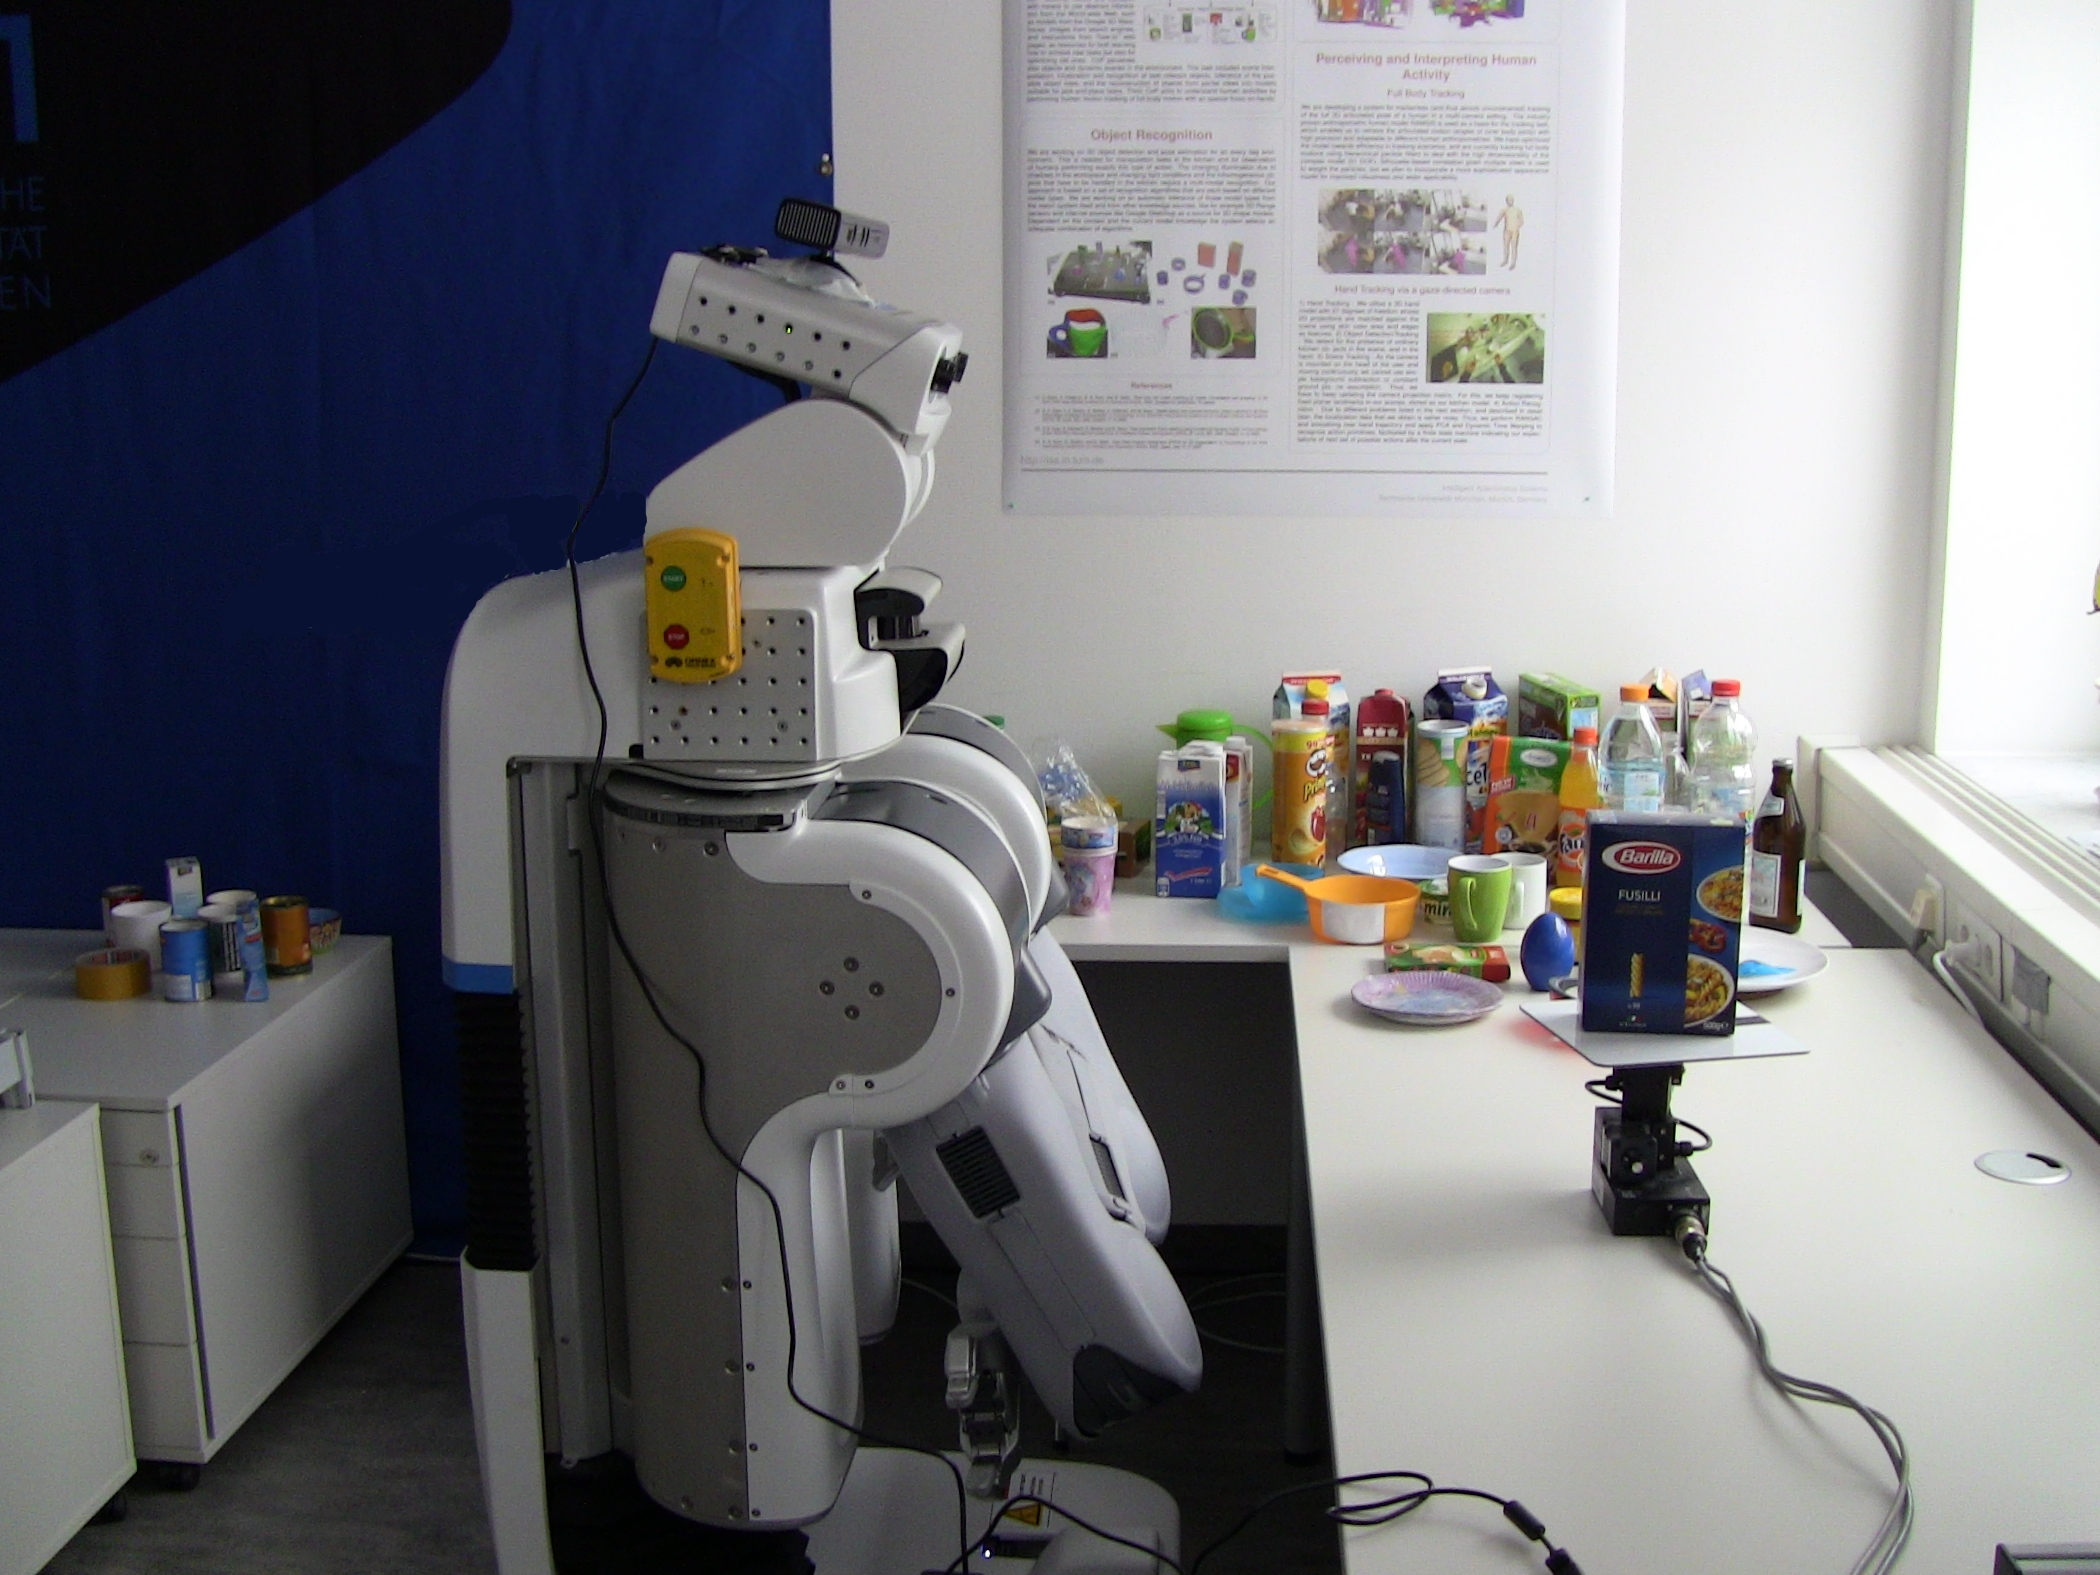
\includegraphics[width=.9\columnwidth]{figures/objects/pr2_rot_table.jpg}
    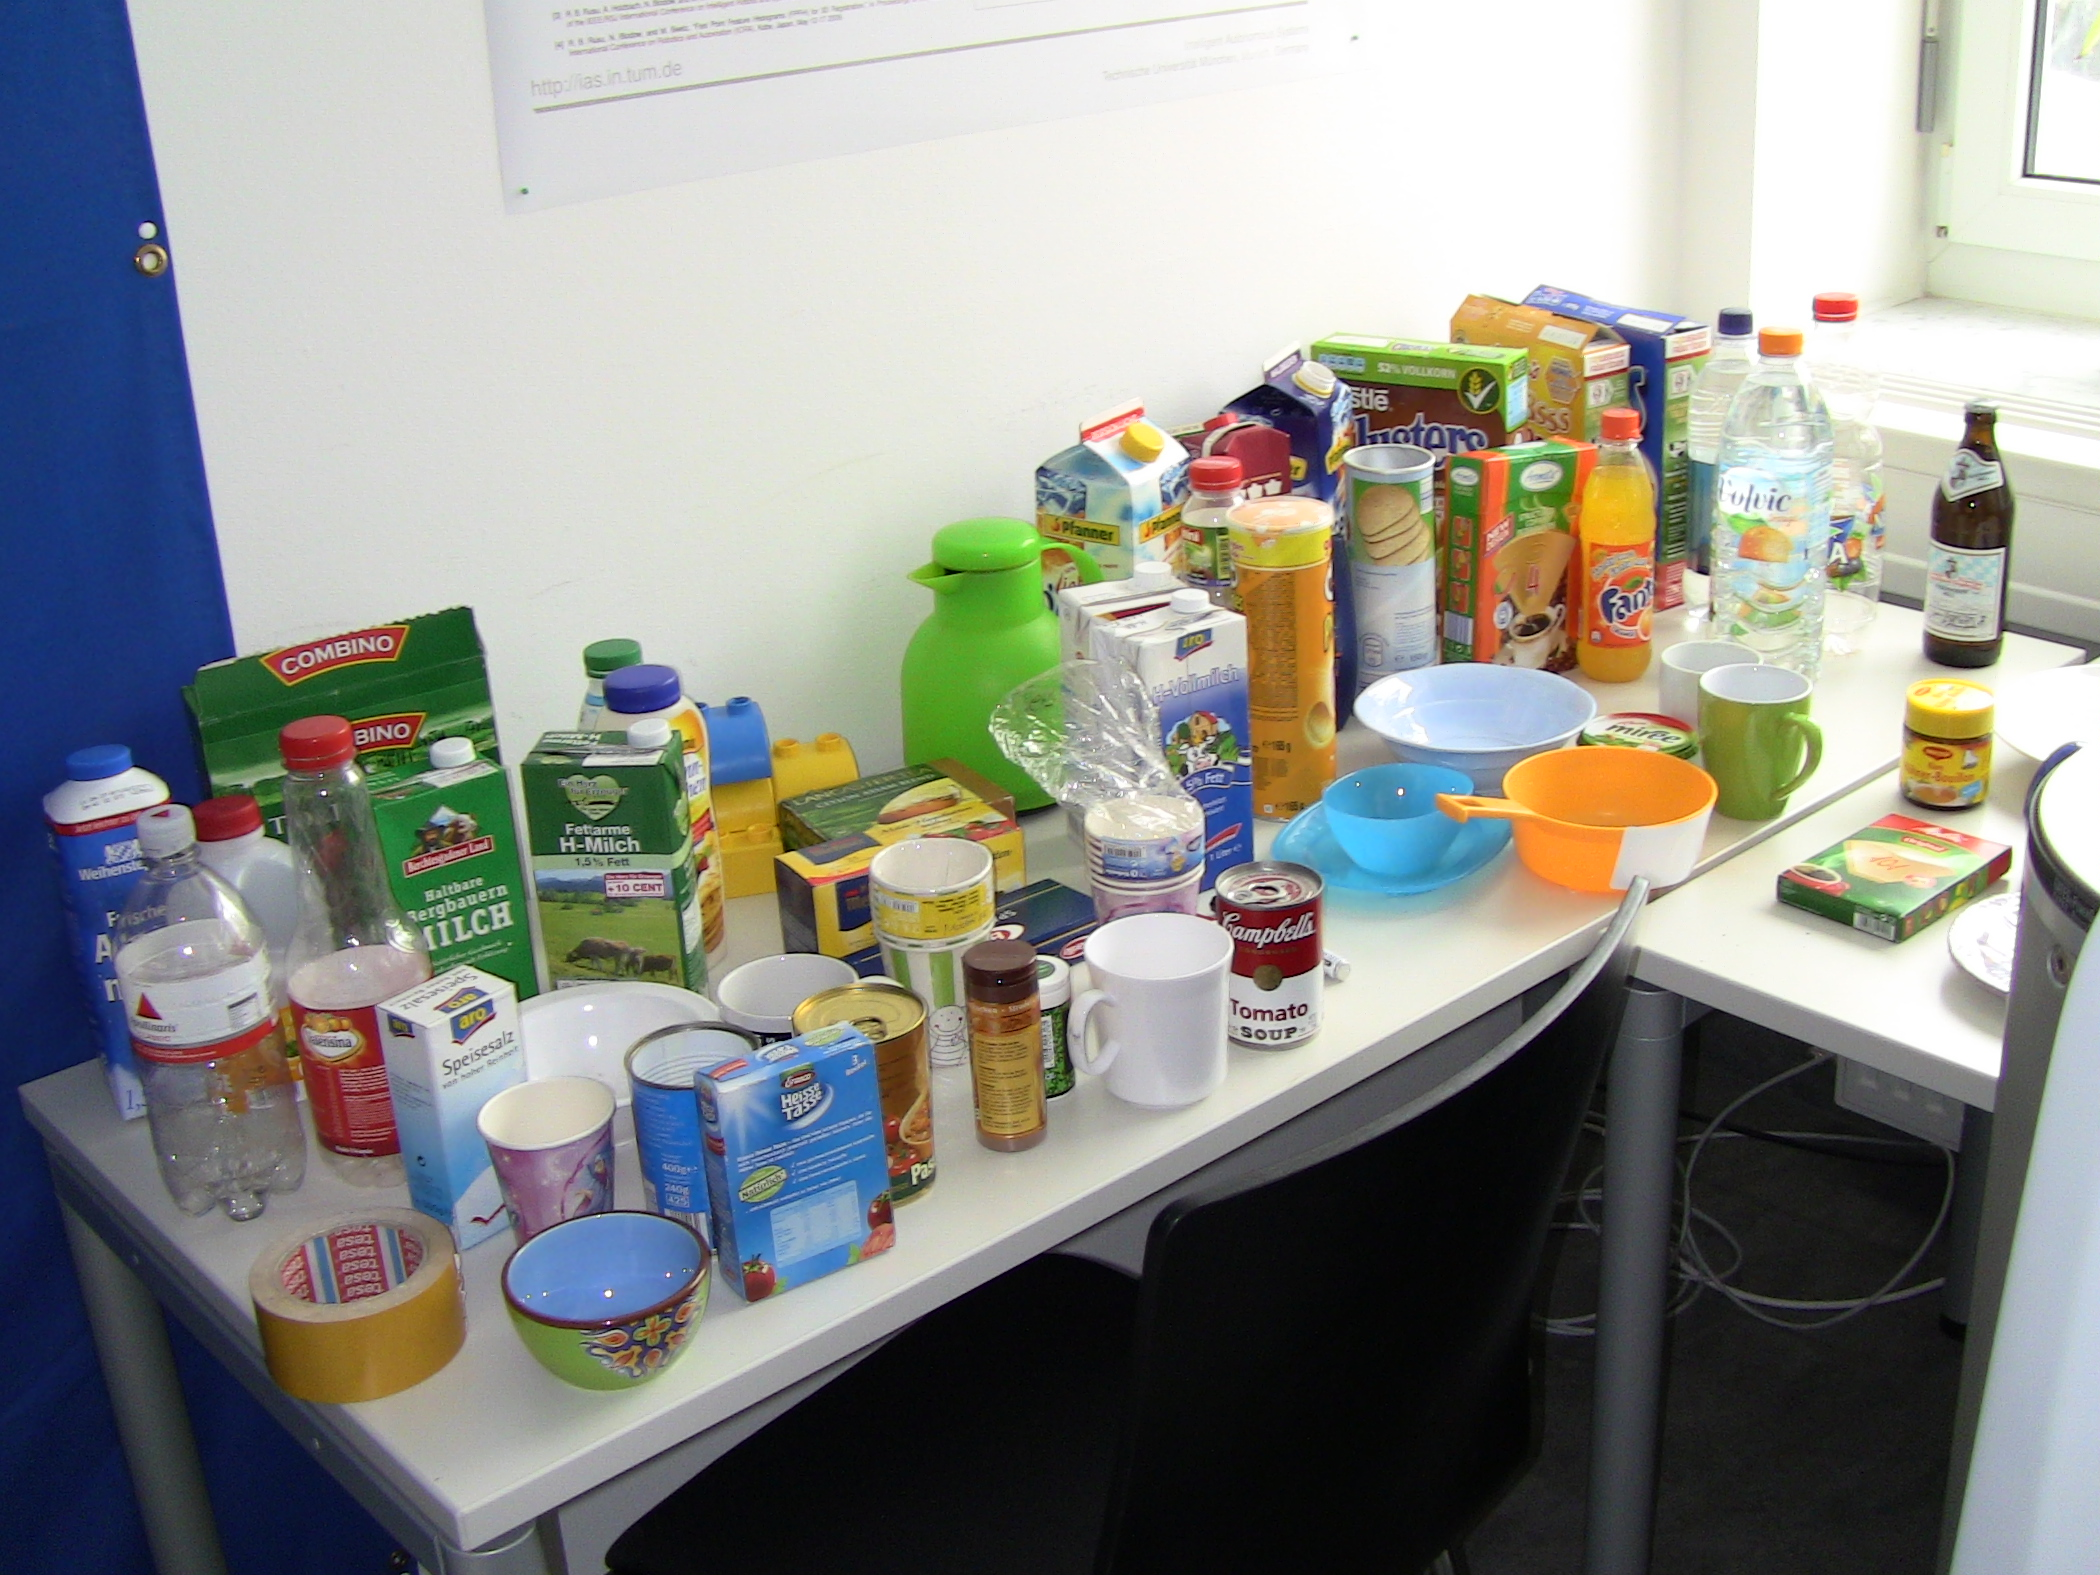
\includegraphics[width=.9\columnwidth]{figures/objects/objects.jpg}
    \caption{Our autonomous service robot (PR2) equipped with a Kinect sensor
    acquiring training data of the objects shown in the bottom image}
    \label{fig:robot}
  \end{center}
\end{figure}

% \subsection{What}
% In this paper, we address the problem of localization and recognition of
% objects of daily use in households. To this effect, we employ a multidimensional
% feature descriptor that captures both the geometrical and visual appearance
% properties of the objects.

The strength of the descriptor lies in its ability to consider geometric and
visual features in a unified manner to facilitate object classification. The two
underlying features have been carefully selected because of their similar structures
and the way they are computed from voxelized 3D data. In this way, their combination is
not a mere concatenation of two different features, but their computation is
performed in a single step because of the common underlying algorithmic
properties. Both features %though independently developed, 
count relations between neighboring voxels, capturing geometric surface type and texture
transitions at the same time.

Further contributions of work presented herein include the ability to deal with
cluttered scenes while eliminating the requirement for region of interest
selection (e.g. horizontal supporting structures) and spatially separable object
clusters. This has been achieved using a moving-bounding-box-based approach, and
a sub-space-matching-based classification scheme (Section
\ref{sec:recognition}). The resulting approach performs at 2 frames per second
while taking into account an object database of 63 different objects
(see Figure~\ref{fig:robot}).

% \subsection{Why}
% In the past, strong features have been proposed in perception for personal robots,
% both working on 2D and 3D data. Prominent examples include
% SIFT~\cite{lowe04distinctive} and SURF~\cite{surf} for camera images, Normal Aligned Radial
% Features (NARF)\cite{steder10irosws} for range images, and several versions of Point Feature
% Histograms (PFH, FPFH)~\cite{Rusu09ICRA} and Viewpoint Feature Histograms
% (VFH)~\cite{vfh} for unordered fully-3D point clouds.
% \todo{Nico proof-read till here}


% Yet it seems that there is none that can capture
% all important and obvious properties (such as geometry and color are)
Lastly, our descriptor can be out-of-the box applied on the data coming out of the 
new sensing technologies such as Kinect device and lays the foundation stone for a
multitude of applications such as later presented recognition of a priori learned object models
(Section~\ref{sec:recognition}). VOSCH also enables equipping of service robots 
(such as PR2 shown in top part of Figure~\ref{fig:robot}) with the 
capabilities to acquire additional object models which furthermore opens ways 
for manipulation tasks in realistic environments under realistic conditions.

\subsection{How}
Since the focus of the paper is on three parts, i.e. i)VOSCH descriptor
construction, ii)database assembly and training of object models and iii)testing,
we solved each of them individually. In the first case we had to unify underlying
structures such that the ColorCHLAC became rotation invariant and GRSD 
additive~\cite{kanezaki2010tvc}. We thus obtained a descriptor histogram with 
137 bins representing the transitions between its different dimensions.
In the second case, we assembled a large database of
object models (Figure~\ref{fig:robot} bottom), by creating a rotating
table using a DP PTU47 pan-tilt unit that is controlled by the robot over the
network. Objects placed on this rotating table were scanned at a given
angle-step ($15^\circ$) and dumped to the disk. The resultant database of
object models was then used to classify objects found in
natural table setting scenes while performing manipulation
tasks. For this third case we also performed a test on objects that were
segmented in the euclidean sense. 

Our approach is realized as part of the Robot Operating System
(ROS)\footnote{\url{http://www.ros.org}} open source initiative, and makes
use of modular and robust components that can be reused on other robotic
systems different than ours.

% \item Combination of view-variant ColorCHLAC and GRSD with the
% normalization of the latter by number 27 (number of transitions)
% \item Combination of view-invariant version of ColorCHLAC and GRSD
% \item Comparisson of Linear Subspace Method and SVM Classifier


\subsection{Performance and Novelty}
Our approach takes 404 seconds for the training of 63 objects and \todo{Y} seconds
for the recognition of already segmented single object. Moving-bounding-box-based
recognition of objects in e.g. cluttered scenes takes 0.5 second as detailed
in Section~\ref{sec:recognition}.

The main novel contributions of this paper are the following:
\begin{itemize}
\item novel, multidimensional descriptor VOSCH that accounts for
geometrical as well as visual appearance  properties of objects in question
\item comparison of classification results for two established classification
frameworks; Linear Subspace Method~\cite{watanabe1973} and Support Vector Machine~\cite{svm99}.
\item an extensive database of objects of daily use captured with the Kinect sensor 
(which we intend to publish after the review process).
\end{itemize}

The remainder of the paper is built as following. After the overview of the related
work in Section~\ref{sec:rl} we present the major system components in Section~\ref{sec:overview}
which is followed by Section~\ref{sec:features} that elaborates on the construction of the
VOSCH descriptor. In Section~\ref{sec:classification} we present the usage of this descriptor
for the classification of objects using two state-of-the-art classification methods which we
then elaborately test and present in Section~\ref{sec:results}. In Section~\ref{sec:conclusion}
we conclude and give the future outlook.

\section{Related Work}
\label{sec:rl}
%\item Color CHLAC (Asako)~\cite{kanezaki2010icra}\cite{kanezaki2010tvc}
% \item textured-spin images~\cite{Johnson_spin_images}
% \item A sparse texture representation using local affine
% regions~\cite{Lazebnik05asparse}
% \item sift-keypoint
% \url{http://www.ros.org/doc/api/pcl/html/sift__keypoint_8h_source.html}
Expressiveness and efficiency of the descriptor are both crucially important for
a real-time object recognition system.  Though there is a trade-off between
these two abilities, it will dramatically improve both of them to select a
proper matching method taking advantage of the characteristics of the
descriptor. In the recent decade a bunch of powerful 2D and 3D descriptors for
recognizing real objects have been developed, however, few of them take into
account the compatibility with the matching method used with them.

SIFT~\cite{lowe04distinctive} descriptor, one of the most well-known 2D
descriptors for object recognition, basically used with detecting keypoints in
scenes and comparing them with those of reference objects to identify the
objects currently observed. A combination of the visual appearance
descriptor and 2D shape is presented by Bosch et al. in~\cite{Bosch07shape}
where they use random forests to achieve around 80\% of classification 
accuracy. Half-way through to 3D domain an effective descriptor
NARF~\cite{steder10irosws}, which detects salient points in range images of
real environments, has recently been developed.  Instead of their dominant
repeatability in point-to-point matching, there still remains difficulty in
cluster-to-cluster matching, which is necessary for identifying each cluster in
environments as an object. This also causes computational expensiveness
especially when the target object database is large. In 3D domain a recently 
developed VFH~\cite{vfh} descriptor was presented as an extension 
of~\cite{Rusu09ICRA}. The feature's discriminative power is boosted up
by an inclusion of viewpoint which on the other side however represents
the deficiency in that it becomes orientation variant. 

There are several approaches that use both geometry and color descriptors to
represent 3D shapes~\cite{park2006}, however, to properly balance these two
different properties is difficult.  Caputo and Dorko~\cite{caputo2002} learned
respective kernels for shape and color representations and combined them for
recognition object, while Huang and Hilton~\cite{huang2009} balanced them by
normalizing bins of shape-color histograms.  Alternative solution for combining
geometry and color information at a proper balance is to extract descriptors
represented by patterns of shape-and-color co-occurrence.  For example, Textured
spin-image~\cite{cortelazzo2006} splits well-known
spin-image~\cite{Johnson_spin_images} descriptors into several layer
corresponding to a given level of luminance. Color-CHLAC~\cite{kanezaki2010icra} 
splits CHLAC~\cite{kobayashi2004} descriptor, which is a histogram of 14 patterns 
depending on relative position of neighboring voxels, into RGB channels and correlation 
space of these channels.  In \cite{kanezaki2010icra} Color-CHLAC descriptor is used as local
descriptors in the training process and as a global descriptor describing each
object cluster in the recognition process, taking advantage of the combination
of linear subspace method and the descriptor's additive property.  We also use
the same approach that uses linear subspace method to enable efficient
processing, with more accuracy achieved by the newly developed histogram-based
descriptor.

\section{System Overview}
\label{sec:overview}
\todo{Dejan}

\section{Feature Estimation}
\label{sec:features}

\subsection{Color CHLAC}
Color-CHLAC descriptor is a high-dimentional vector measuring the summation of the multiplicated RGB values of neighboring voxels around a voxel grid of arbitrary size. 
Each bin in a Color-CHLAC descriptor is differentiated by RGB color space and the relative position of the two neighboring voxels. 
Let $\bm{x}=(x,y,z)^T$ be the position of a voxel, $p(\bm{x})$ be the flag for occupancy of the voxel, 
 and $r(\bm{x})$, $g(\bm{x})$ and $b(\bm{x})$ be its RGB values normalized between 0 and 1, respectively. 
By defining $r'(\bm{x}) \equiv 1 - r(\bm{x})$, $g'(\bm{x}) \equiv 1 - g(\bm{x})$ and $b'(\bm{x}) \equiv 1 - b(\bm{x})$, 
    a voxel status $\bm{f}(\bm{x})\in R^6$ is defined as follows: 
%\vspace{-2mm}
\begin{eqnarray*}
  \label{eq:voxel}
%  \hspace{-1mm}
  \bm{f}({\bm x})\hspace{-1mm}=\hspace{-1mm}\left\{
  \begin{array}{cc}
    \hspace{-1mm}
    (r({\bm x})\hspace{1mm} r'({\bm x}) \hspace{1mm}g({\bm x}) \hspace{1mm}g'({\bm x}) \hspace{1mm}b({\bm x}) \hspace{1mm}b'({\bm x}))^T & \hspace{-2mm}(p({\bm x})\hspace{-1mm}=\hspace{-1mm}1) \\
    (0\hspace{1mm}0\hspace{1mm}0\hspace{1mm}0\hspace{1mm}0\hspace{1mm}0)^T & \hspace{-2mm}(p({\bm x})\hspace{-1mm}=\hspace{-1mm}0)
  \end{array}\right.
\end{eqnarray*}
%
%Color-CHLAC features are the integral of $\bm{f}(\bm{x})$ or correlations of $\bm{f}(\bm{x})$ between neighboring voxels.
Letting ${\bm a}$ be a displacement vector from the reference voxel to its neighboring voxel, 
   the containts of a Color-CHLAC descriptor are calculated by following equations:
\begin{equation}\label{eq:0th}
  {\bm q} = \sum \bm{f}({\bm x})
\end{equation}
\begin{equation}\label{eq:0th_1}
  {\bm q} = \sum \bm{f}({\bm x}) \hspace{1mm}\bm{f}^T({\bm x}) \\
\end{equation}
\begin{equation}\label{eq:1st}
  {\bm q}({\bm a}) = \sum \bm{f}({\bm x}) \hspace{1mm}\bm{f}^T({\bm x}+{\bm a}) \\
\end{equation}
%
Since these values are summed up around a voxel grid, there is a redundancy that checks the same value twice over symmetric pairs of ${\bm a}$. 
As the result, the number of variations in ${\bm a}$ is 13, which is a half of all the 26 neighbors.
The matix computed by (\ref{eq:1st}) is expanded into a column vector of 36 elements.
Therefore the dimension of the vector calculated by (\ref{eq:0th}) is 6, while that by (\ref{eq:1st}) is 468 (=36*13).
 
 Color-CHLAC descriptor is also computed from a voxel grid where $r(\bm{x})$, $g(\bm{x})$ and $b(\bm{x})$ are binarized as a pre-processing of features extraction. See details in \cite{kanezaki2010icra}. 
 Excluding redundant elements, the dimension of Color-CHLAC features calculated by (\ref{eq:0th_1}) is 12 if color values are binarized, and 21 otherwise. 
 Finally a full Color-CHLAC vector is obtained by concatenating the two vectors from binarized color voxel data and from original color voxel data. 
 Then the dimension of Color-CHLAC feature vector becomes 981 (=6+6+468+468+12+21).
 \todo{Rotation-invariant version in VOSCH-RGBD from here.}
 To produce a new descriptor based on Color-CHLAC and GRSD, we refined Color-CHLAC descriptor to be rotation-invariant by bringing all the 13 different vectors given by (\ref{eq:1st}) together. 
 Then the dimention of this descriptor becomes 117 (=6+6+36+36+12+21). 
 This is the similar way that GRSD takes, where the transitions between the reference voxel and all the 26 nighbors are combined together. 
 Therefore this refined Color-CHLAC descriptor is well concerted with GRSD, gives significant robustness to rotation and still shows a powerful expressivity for color textures.

\subsection{GRSD}
%
GRSD is a histogram, that counts the number of transitions between different types of voxels.
This approach is similar to ColorCHLAC, but in order to efficiently merge the two features,
the original GRSD has to be simplified. As presented in \cite{GRSD10Humanoids} we were using
ray-tracing in order to find transitions between surface types of voxels. To merge the features,
ray-tracing was abandoned for simple checks of neighboring voxels, and the feature is no longer normalized.

These modifications allow us to create histograms which, like ColorCHLAC, are roughly additive.
If we break up objects into reasonable sizes, its histogram can be approximated by the sum of the
histograms of its partitioning. Unlike in ColorCHLAC, free space is considered, but we are looking
at the neighbors of occupied voxels only.

As the feature is rotation invariant, the number of bins $b$ depends on the number of possible surface types $s$ (including emph-empty):
\begin{equation}
b=\frac{s(s+1)}{2}-s
\end{equation}
Previously only predefined surface types with an intuitive description were used (cylinder, sphere, plane, rim and corner),
based on an estimation of the radii of the 2 principal curves defining the surface, $r_{min}$ and $r_{max}$ \cite{Marton10IROS}.
Since these values have physical meaning, we can categorize surfaces into predefined types, but
\todo{now we are dividing, so we get more surface types, chosen to roughly match ColorCHLAC to have the same "weighting"}

Once all voxels are annotated locally using a geometric class, our
processing pipeline constructs a global feature by counting the transitions
between these local labels (and free space), as shown in Figure\todo{~\ref{fig:grsd}}.
Since we do not use ray-casting but consider only the direct neighbors
of each occupied cell, the computation of this \emph{simplified} GRSD is much faster.

\begin{figure}[htb!]
  \begin{center}
    \includegraphics[width=.48\columnwidth]{figures/colorCHLAC/artificial/purple.png}
    \includegraphics[width=.48\columnwidth]{figures/colorCHLAC/artificial/torus.png}
    \caption{Examples of GRSD-ColorCHLAC histograms. Left: different categories
of objects result in having different first 20 bins of the respective histogram.
Right: different colors of the same category of an object have different 137 last bins
of the histogram}
    \label{fig:grsd_cchlac}
  \end{center}
\end{figure}

\subsection{Comparison}
%
Same approach (if using rotation invariant ColorCHLAC), but different things are counted (color vs surface type). Also, GRSD considers free space as well.
\begin{figure}[htb!]
  \begin{center}
    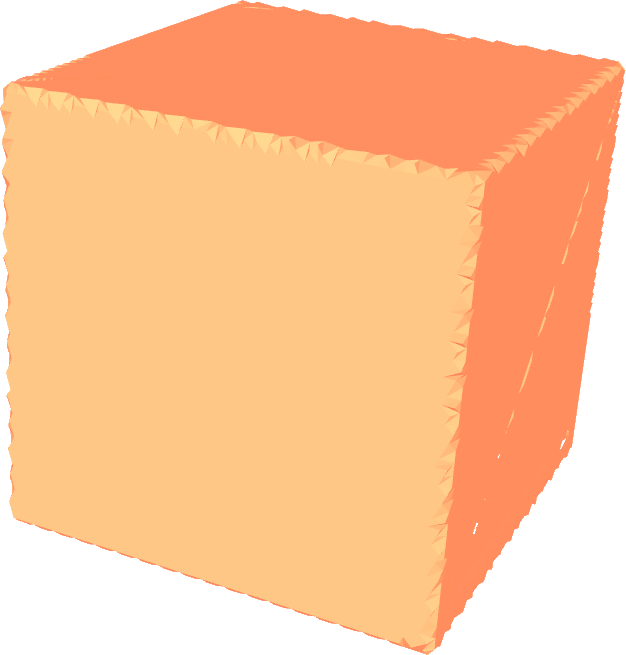
\includegraphics[width=.3\columnwidth]{figures/comparison/cube.png}
    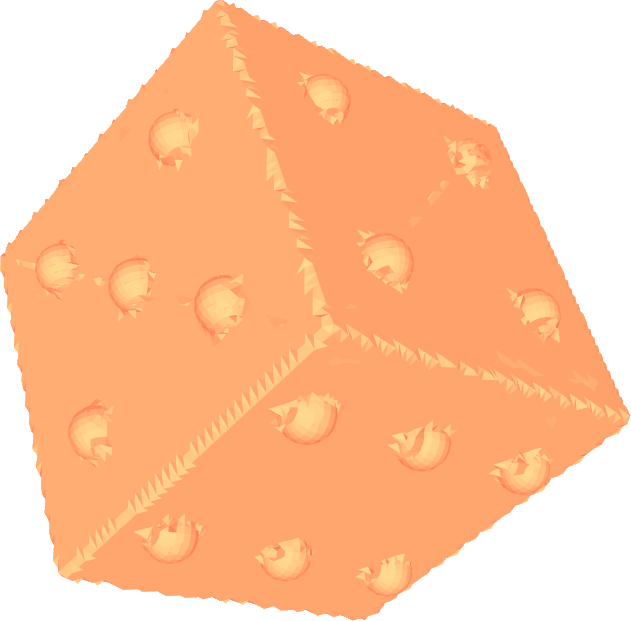
\includegraphics[width=.32\columnwidth]{figures/comparison/dice1.png}
    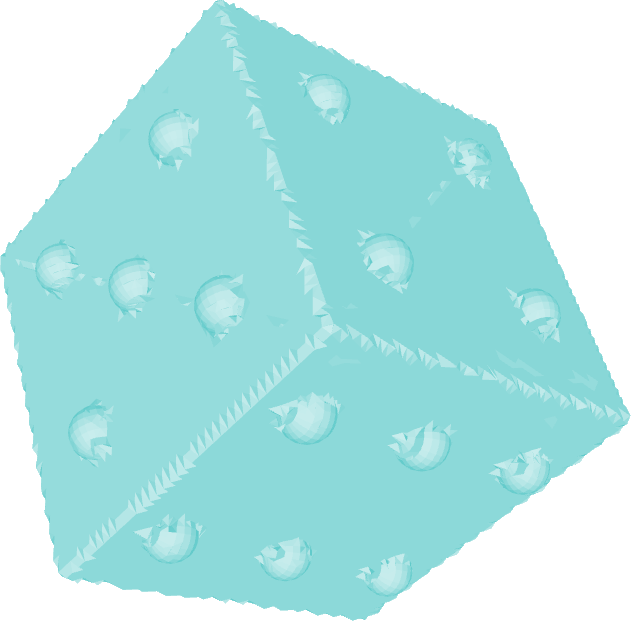
\includegraphics[width=.32\columnwidth]{figures/comparison/dice2.png}
    \caption{Color-CHLAC: can not differentiate the dice from the cube. GRSD: can not differentiate the different colors. Combination solves both.}
    \label{fig:comparison}
  \end{center}
\vspace{-2ex}
\end{figure}

\section{Classification Methods}
\label{sec:classification}
\subsection{Linear Subspace Method}
\label{sec:subspace}
\todo{Asako: revise this subsection.}
\subsubsection{Creating subspaces of objects in a database}
First, the voxel data of each object in a database is subdivided into a voxel grid of a certain size,
    e.g. $10 \times 10 \times 10$ voxels.
Suppose the $i$-th object in the database is divided into $M_i$ subdivisions.
Then $M_i$ Color-CHLAC feature vectors are extracted.
To achieve robustness to rotation,
    features extraction is repeated with various poses of the object.
The feature vector of an object which is rotated by 90 degrees can be obtained rapidly
    through a simple exchange of the elements of the feature vector in the initial posture.
This is possible because each displacement vector in Fig.~\ref{fig:displacement_vectors}
    is equivalent to another, rotated by 90 degrees.
In this paper, we use this 90 degrees rotation in 24 ways,
    and rotations of 30 and 60 degrees in 21 ways,
    resulting in achieving 504($=24 \times 21$) varieties of postures for an object.
Therefore, the number of Color-CHLAC feature vectors
    generated from each object is $N_i \equiv 504M_i$.

We represent a Color-CHLAC feature vector compressed by PCA as $\bm{z}_t \in R^d, t=1,2,...N_i$,
    where $d$ is the dimension of a compressed feature vector.
The auto-correlation matrix of these feature vectors is calculated by the following equation:
\begin{eqnarray*}
  %\hspace{-1mm}
  R_i = \frac{1}{N_i} \sum^{N_i}_{t=1} \bm{z}_t \bm{z}_t^T
\end{eqnarray*}
The eigenvectors of $R_i$ are then computed by solving the eigenvector problem.
Finally, the bases of the subspace of the $i$-th object in the database, $P_i \equiv (\bm{v}_{i1} \bm{v}_{i2} ... \bm{v}_{ir})$,
    are obtained as the $r$ eigenvectors of largest eigenvalue.

\subsubsection{Calculation of Similarity}
The first step in the recognition process is to compute
    one Color-CHLAC feature vector from the whole of a query part in a 3D scene. % ???
Then the compressed feature vector $\bm{z}$ is computed using the projection matrix which is
    generated from all Color-CHLAC feature vectors of each database object in the pre-processing phase.
Let the similarity between the query part and the $i$-th object in the database be $y_i$.
$y_i$ is defined as the cosine of the angle between $\bm{z}$ and the subspace of the $i$-th object.
$y_i$ is calculated by the following equation:
\begin{eqnarray}\label{eq:y_calc}
  %\hspace{-1mm}
  y_i = \frac{\| P_i^T \bm{z} \|}{\| \bm{z} \|}
\end{eqnarray}


\subsection{Support Vector Machine-based Classification}
\todo{Zoli}

\section{Results}
\label{sec:results}
\subsection{Feature Extraction}
Synthetic Data: (49 views of objects), 0.0000363877551020408 sec/point, average number of points: 19124
Real Data (1512 views of objects), 0.0000577394179894179  sec/point,  average number of points: 4632

\subsection{Synthetic Data}

\begin{table*}[ht]
\newcommand{\mc}[3]{\multicolumn{#1}{#2}{#3}}
\definecolor{tcA}{rgb}{0.784314,0.784314,0.784314}
\begin{center}
\begin{tabular}{|c|c|c|c|c|c|c|c|c|c|}\hline
% use packages: color,colortbl
\rowcolor{tcA} \textbf{} & \textbf{} & \mc{2}{>{\columncolor{tcA}}c|}{\textbf{GRSD}} & \mc{2}{>{\columncolor{tcA}}c|}{\textbf{Color-CHLAC}} & \mc{2}{>{\columncolor{tcA}}c|}{\textbf{MERGED}} & \mc{2}{>{\columncolor{tcA}}c|}{\textbf{VOSCH}}\\
\cline{3-10}
\rowcolor{tcA} \textbf{Noise STD} & \textbf{Rotation} & \textbf{LSM} & \textbf{SVM} & \textbf{LSM} & \textbf{SVM} & \textbf{LSM} & \textbf{SVM} & \textbf{LSM} & \textbf{SVM}\\
\hline
\mc{1}{|>{\columncolor{tcA}}c|}{\textbf{0.5}} & \mc{1}{>{\columncolor{tcA}}c|}{\textbf{None:}} &  & 14.2857\% &  & 100\% &  & 100\% &  & 100\% \\
\rowcolor{tcA} \textbf{mm} & \textbf{Random:} &  & 12.6531\% &  & 70.2041\% &  & 79.5918\% &  & 91.4286\% \\
\hline
\mc{1}{|>{\columncolor{tcA}}c|}{\textbf{1.0}} & \mc{1}{>{\columncolor{tcA}}c|}{\textbf{None:}} &  & 14.2857\% &  & 77.1429\% &  & 85.7143\% &  & 100\% \\
\rowcolor{tcA} \textbf{mm} & \textbf{Random:} &  & 14.2857\% &  & 65.7143\% &  & 78.7755\% &  & 99.5918\% \\
\hline
\mc{1}{|>{\columncolor{tcA}}c|}{\textbf{1.5}} & \mc{1}{>{\columncolor{tcA}}c|}{\textbf{None:}} &  & 13.0612\% &  & 28.5714\% &  & 85.7143\% &  & 91.4286\% \\
\rowcolor{tcA} \textbf{mm} & \textbf{Random:} &  & 13.0612\% &  & 26.1224\% &  & 82.449\% &  & 90.6122\% \\
\hline
\mc{1}{|>{\columncolor{tcA}}c|}{\textbf{2.0}} & \mc{1}{>{\columncolor{tcA}}c|}{\textbf{None:}} &  & 12.2449\% &  & 28.5714\% &  & 85.7143\% &  & 85.7143\% \\
\rowcolor{tcA} \textbf{mm} & \textbf{Random:} &  & 12.2449\% &  & 20.8163\% &  & 85.7143\% &  & 85.7143\% \\
\hline
\mc{1}{|>{\columncolor{tcA}}c|}{\textbf{2.5}} & \mc{1}{>{\columncolor{tcA}}c|}{\textbf{None:}} &  & 10.2041\% &  & 28.5714\% &  & 57.1429\% &  & 71.4286\% \\
\rowcolor{tcA} \textbf{mm} & \textbf{Random:} &  & 10.2041\% &  & 25.7143\% &  & 57.1429\% &  & 71.4286\% \\
\hline
\mc{1}{|>{\columncolor{tcA}}c|}{\textbf{3.0}} & \mc{1}{>{\columncolor{tcA}}c|}{\textbf{None:}} &  & 10.2041\% &  & 28.5714\% &  & 57.1429\% &  & 71.4286\% \\
\rowcolor{tcA} \textbf{mm} & \textbf{Random:} &  & 10.2041\% &  & 28.5714\% &  & 55.5102\% &  & 71.4286\% \\
\hline
\mc{1}{|>{\columncolor{tcA}}c|}{\textbf{3.5}} & \mc{1}{>{\columncolor{tcA}}c|}{\textbf{None:}} &  & 10.2041\% &  & 28.5714\% &  & 57.1429\% &  & 71.4286\% \\
\rowcolor{tcA} \textbf{mm} & \textbf{Random:} &  & 10.2041\% &  & 28.5714\% &  & 45.3061\% &  & 71.4286\% \\
\hline
\mc{1}{|>{\columncolor{tcA}}c|}{\textbf{4.0}} & \mc{1}{>{\columncolor{tcA}}c|}{\textbf{None:}} &  & 8.57143\% &  & 28.5714\% &  & 43.2653\% &  & 68.5714\% \\
\rowcolor{tcA} \textbf{mm} & \textbf{Random} &  & 8.57143\% &  & 28.5714\% &  & 42.8571\% &  & 70.2041\% \\
\hline
\mc{1}{|>{\columncolor{tcA}}c|}{\textbf{4.5}} & \mc{1}{>{\columncolor{tcA}}c|}{\textbf{None:}} &  & 8.16327\% &  & 28.5714\% &  & 42.8571\% &  & 74.2857\% \\
\rowcolor{tcA} \textbf{mm} & \textbf{Random:} &  & 7.7551\% &  & 28.5714\% &  & 44.898\% &  & 68.1633\% \\
\hline
\mc{1}{|>{\columncolor{tcA}}c|}{\textbf{5.0}} & \mc{1}{>{\columncolor{tcA}}c|}{\textbf{None:}} &  & 5.71429\% &  & 28.5714\% &  & 53.4694\% &  & 53.8776\% \\
\rowcolor{tcA} \textbf{mm} & \textbf{Random:} &  & 6.12245\% &  & 28.5714\% &  & 52.6531\% &  & 52.2449\% \\
\hline
\end{tabular}
\caption{Comparison of Features and Classifiers}
\label{tbl:synthetic}
\end{center}
\end{table*}


\subsection{Real Data}
\subsubsection{Data Aquisition and Training}

Our database of 3D objects, available at \url{http://semantic-3d.cs.tum.edu},
(\todo{upload}) was obtained using the Kinect sensor.

The set of objects (see Figure~\ref{fig:robot}) encompasses the ones commonly used
in a typical household environment (mugs, utensils, books, etc) and is envisioned for a
larger expansion in the future.  In a pursue to account for a wide variety
of view angles, we rotated the objects on the rotating table with a given
angle-step ($15^\circ$ in the preliminary version) and acquired partial
snapshots from a human-eye perspective, i.e. the ones that the best
approximate the robot's view point during its working cycle.  We consider
this to be an important point as opposed to similar initiatives (e.g.,
\cite{kit}) where the datasets are acquired using high-precision but
non-affordable, fixed sensors, and thus not usable for applications such as ours.

\begin{figure}[htb!]
  \begin{center}
    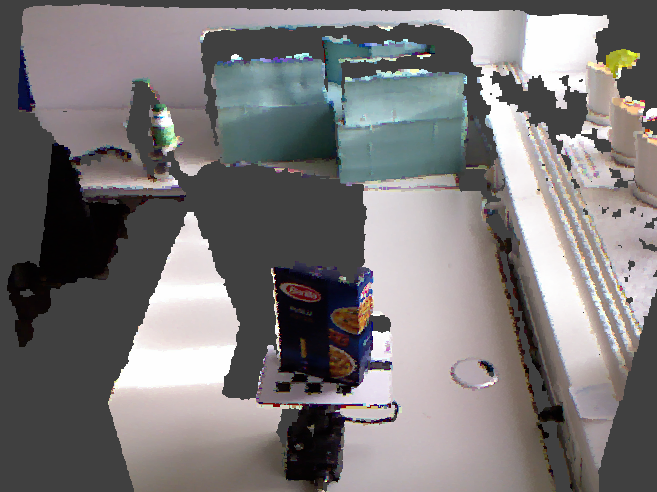
\includegraphics[width=.45\columnwidth]{figures/rot_table/barilla.png}
\hfill
    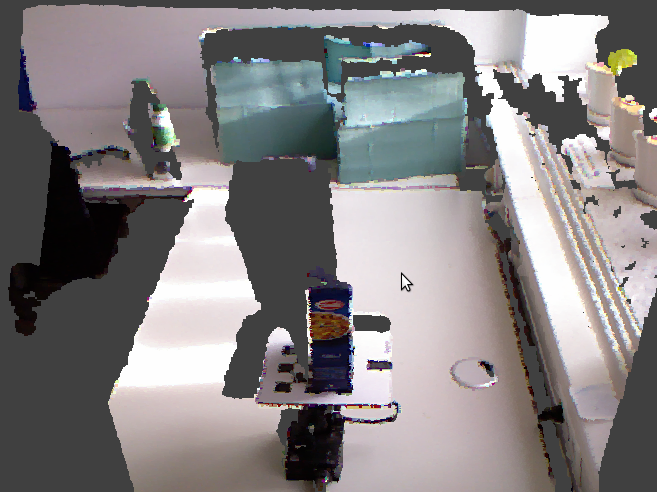
\includegraphics[width=.45\columnwidth]{figures/rot_table/barilla1.png} \\
    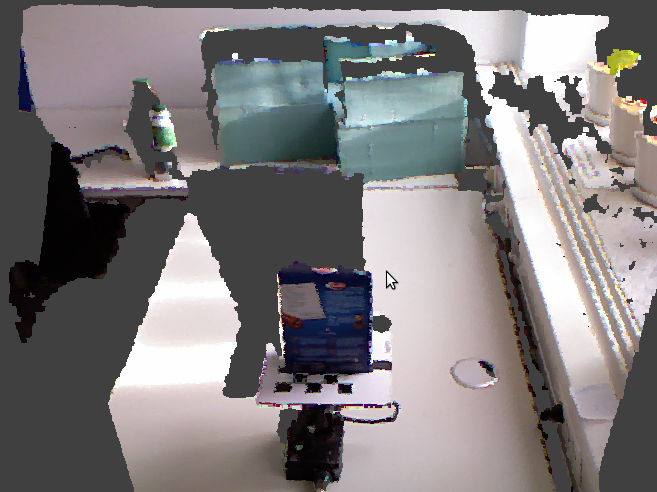
\includegraphics[width=.45\columnwidth]{figures/rot_table/barilla2.png}
\caption{Acquisition of Training Data}
    \label{fig:data_acquisition}
  \end{center}
\end{figure}

\begin{figure}[htb!]
  \begin{center}
    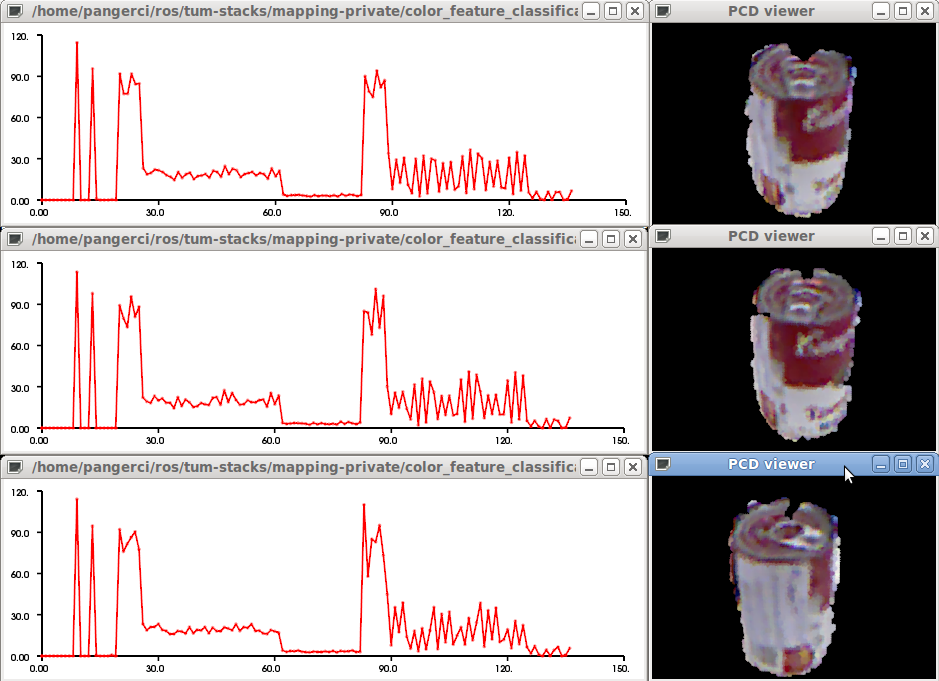
\includegraphics[width=.9\columnwidth]{figures/colorCHLAC/real/tomato/tomato_hist_pcd.png}
    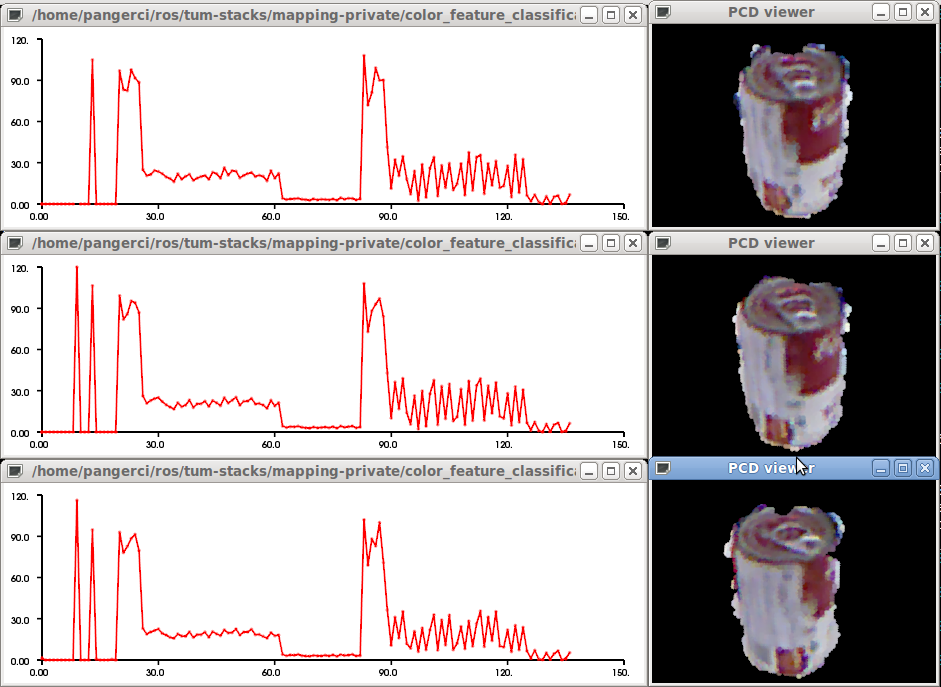
\includegraphics[width=.9\columnwidth]{figures/colorCHLAC/real/tomato/tomato_hist_pcd2.png}
    \caption{Examples of GRSD-ColorCHLAC histograms for a Tomato Soup can.}
    \label{fig:grsd_colorchlac_tomato}
  \end{center}
\end{figure}


\subsubsection{Leave-one-out Test}
\todo{ALL}

\subsubsection{Find One Object Test}
\todo{Prove it works for a)textured objects, b)texture-less objects, c)objects with different shapes, 
d)varying lighting conditions}
%\todo{Dejan}

\subsection{Object Detection Pipeline (in Clutter)}
\label{sec:recognition}
We applied our object recognition method on an object detection scheme in a cluttered environment.
The system computes the similarities between each target object and all rectangular-solid sub-regions in the environment, and then it outputs all the regions that have higher similarities than a certain threshold as the candidates of the target object.
Each sub-region has the same size as that of the bounding box of the target object.
To accelerate feature extraction from the sub-regions, we used ``Integral Feature Table''~\cite{kanezaki2010tvc}, which is a simple extension of ``Integral Image''~\cite{viola2001} from 2D to 3D.
The ``Integral Feature Table'' $\bm{I}(x,y,z)$ is defined as the $d$-dimensional compressed feature vector extracted from the voxel area
    ranging from $(0,0,0)$ to $(x,y,z)$.
Let the feature vector of the voxel area with $x$ ranging from $x_1$ to $x_2$,
    $y$ ranging from $y_1$ to $y_2$, and $z$ ranging from $z_1$ to $z_2$, be $\bm{F}(x_1,y_1,z_1,x_2,y_2,z_2)$.
This is computed by the following equation:
\begin{eqnarray*}\label{eq:sat}
\bm{F}(x_1,y_1,z_1,x_2,y_2,z_2) = \bm{I}(x_2,y_2,z_2) - \bm{I}(x_1,y_2,z_2)
                           \\ - \bm{I}(x_2,y_1,z_2) - \bm{I}(x_2,y_2,z_1)
                           \\ + \bm{I}(x_1,y_1,z_2) + \bm{I}(x_1,y_2,z_1)
                           \\ + \bm{I}(x_2,y_1,z_1) - \bm{I}(x_1,y_1,z_1)
\end{eqnarray*}
Using the ``Integral Feature Table'', $\bm{F}(x_1,y_1,z_1,x_2,y_2,z_2)$ can always be computed by adding the 8 cached feature vectors,
    regardless of the size of the target object.
Note that this is not effective when the number of sub-regions included in the detection box is smaller than 8.
Within the large color voxel data of an environment,
   only the voxels on the surface of each object have RGB values, while other voxels have the empty property.
This means that the object detection process can be accelerated by skipping empty regions.
Similarly to the ``Integral Feature Table'', we create a table that stores
   the number of voxels with the occupied property, in the area ranging from $(0,0,0)$ to $(x,y,z)$.
Using this table, the number of voxels with the occupied property in the detection box can be computed quickly by adding 8 scalar values.
If the number is less than a certain threshold $h$,
   the system skips the similarity calculation and moves the detection box forwards.
In this work, we set $h$ to the minimum value of the occupied voxel number in the training samples of the target object.

\todo{Asako: description for the results}


\begin{figure}[htb!]
  \begin{center}
    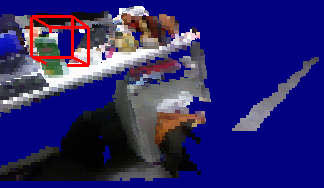
\includegraphics[width=.45\columnwidth]{figures/colorCHLAC/detection7.png}
\hfill
    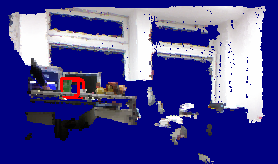
\includegraphics[width=.45\columnwidth]{figures/colorCHLAC/detection5.png} \\
\hfill
    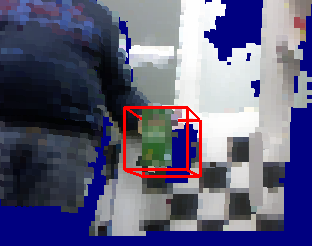
\includegraphics[width=.9\columnwidth]{figures/colorCHLAC/detection2.png}
\caption{An example of the detection of tetrahedral package of milk}
    \label{fig:milk_testing}
  \end{center}
\end{figure}


\section{Conclusions and Future Work}
\label{sec:conclusion}
\todo{ALL}

% \section*{Acknowledgments}
% This work was supported by the DFG cluster of excellence \emph{CoTeSys} (Cognition for Technical Systems).\\
% \todo{Asako: Do we need to ackknowledge someone from ISI Lab?}
% %% Use plainnat to work nicely with natbib.

\bibliographystyle{plainnat}
\bibliography{references}

\end{document}


%TODO:
%Check the original template and see what the meant with the hyperlinks
